\documentclass[border=3pt]{standalone}
% Preâmbulo compartilhado pelos diagramas TikZ da aula 4 de Navegação (Representação de Mapas)
\usepackage[T1]{fontenc}
\usepackage[utf8]{inputenc}
\usepackage{lmodern}
\usepackage{amsmath}
\usepackage{xcolor}
\usepackage{tikz}
\usetikzlibrary{arrows.meta,angles,quotes,decorations.pathmorphing,decorations.pathreplacing,calc,
                positioning,shapes.geometric,shapes.misc,backgrounds,fit,
                math}

% Paleta (mesma dos SVGs originais)
\definecolor{dblue}{HTML}{2A5B8C}
\definecolor{dorange}{HTML}{B3541E}
\definecolor{dgreen}{HTML}{4A7C59}
\definecolor{dred}{HTML}{9C4B4B}
\definecolor{dcream}{HTML}{F4F1EA}
\definecolor{dshade}{HTML}{DDD7C9}

% Função gaussiana (não normalizada por padrão de escala visual)
\pgfmathdeclarefunction{gauss}{3}{%
  \pgfmathparse{1/(#3*sqrt(2*pi))*exp(-((#1-#2)^2)/(2*#3^2))}%
}

% Estilos comuns (prefixo d... para não colidir com chaves internas do pgf)
\tikzset{
  >={Stealth[length=2mm]},
  dguide/.style={gray!55, dashed, line width=0.4pt},
  daxis/.style={gray!60, line width=0.7pt, ->},
  dbody/.style={fill=black!3, draw=black!80, line width=1pt},
  dacc/.style={draw=dblue, line width=1pt},
  dlbl/.style={black!55, font=\small},
  dsub/.style={black!45, font=\footnotesize},
  dstate/.style={circle, draw=black!80, fill=dcream, line width=1pt,
                 minimum size=17mm, font=\large, inner sep=1pt},
  dobs/.style={circle, draw=black!80, fill=dshade, line width=1pt,
               minimum size=14mm, font=\large, inner sep=1pt},
  dbox/.style={rounded corners=2pt, draw=black!80, fill=dcream, line width=1pt,
               align=center, inner sep=6pt},
  dop/.style={circle, draw=black!80, fill=white, line width=1pt,
              minimum size=6mm, inner sep=0pt, font=\small},
  dtrans/.style={->, dblue, line width=1pt},
  dmeas/.style={->, dorange, line width=1pt},
  dcurve/.style={line width=1pt, dblue},
  dcurveb/.style={line width=1.4pt, dorange},
}

\begin{document}
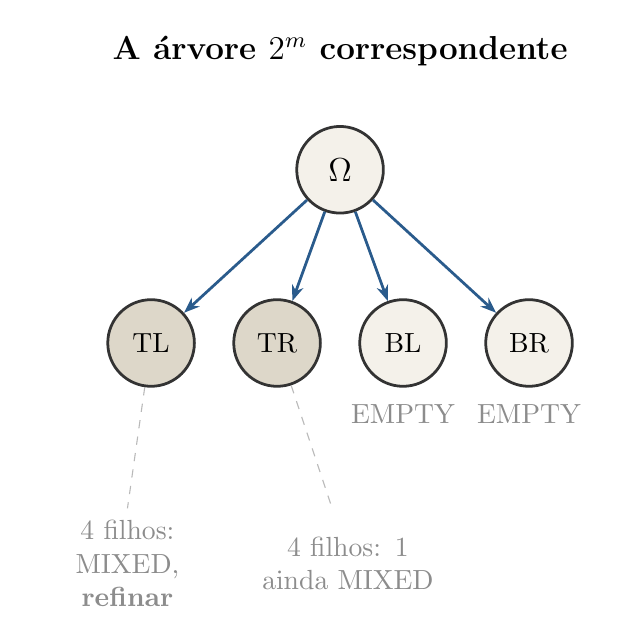
\begin{tikzpicture}[x=1cm,y=1cm]

  % ---------- Painel B: árvore (esquemática) ----------
  \begin{scope}
    \node[font=\bfseries\large] at (3.0,8.5) {A árvore $2^m$ correspondente};

    \node[dstate, minimum size=11mm, font=\large] (root) at (3.0,7.0) {$\Omega$};

    \node[dobs, minimum size=11mm, fill=dshade, font=\normalsize] (tl) at (0.6,4.8) {TL};
    \node[dobs, minimum size=11mm, fill=dshade, font=\normalsize] (tr) at (2.2,4.8) {TR};
    \node[dobs, minimum size=11mm, fill=dcream, font=\normalsize] (bl) at (3.8,4.8) {BL};
    \node[dobs, minimum size=11mm, fill=dcream, font=\normalsize] (br) at (5.4,4.8) {BR};
    \draw[dtrans] (root) -- (tl);
    \draw[dtrans] (root) -- (tr);
    \draw[dtrans] (root) -- (bl);
    \draw[dtrans] (root) -- (br);
    \node[dsub, font=\normalsize] at (3.8,3.9) {EMPTY};
    \node[dsub, font=\normalsize] at (5.4,3.9) {EMPTY};

    \draw[dguide] (tl) -- (0.3,2.7);
    \draw[dguide] (tr) -- (2.9,2.7);
    \node[dsub, font=\normalsize, align=center, text width=2.3cm] at (0.3,2.0) {4 filhos: MIXED, \textbf{refinar}};
    \node[dsub, font=\normalsize, align=center, text width=2.3cm] at (3.1,2.0) {4 filhos: 1 ainda MIXED};

      \end{scope}


\end{tikzpicture}
\end{document}
